\newpage
\chapter{The Large Hadron Collider and the ATLAS detector}
\label{LHC&ATLAS}
\textcolor{red}{ This chapter will include :
\begin{itemize}
    \item LHC description and how it works
    \item different LHC points 
    \item focus on ATLAS as main experiment
    \item focus on EM and H calorimeters 
\end{itemize}
Copy past from other thesis!
} \\
The physics described in this thesis exclusively uses data collected by the ATLAS (A Toroidal LHC Apparatus) detector raised from high-energy proton-proton collisions, accelerated by the Large Hadron Collider (LHC). In terms of achievable centre-of-mass energy, LHC is currently the most powerful particle accelerator on Earth. The structure, parameters and principles of LHC and ATLAS, besides the complex sub-detecting system introduced in this chapter.

\section{The Large Hadron Collider}
\label{chap2:LHC}
LHC is a circular accelerator of hadrons with a circumference of 27 kilometers. It was designed to accelerate and collide proton beams with a centre-of-mass energy up to 14 TeV as well as heavy ions, in particular lead nuclei (Pb), at 2.3 TeV per nucleon. Inside this circular accelerator a set of protons (or nucleons) so-called bunch racing clockwise at near the speed of light (99.9999991\%) crashes into an other bunch speeding anticlockwise. The energy involved in the collisions is so great that, in a sub-microscopic region at the heart of the collisions, it briefly generates conditions similar to those that occurred shortly after the birth of the Universe. This machine is installed in the 27 km tunnel, located underground between 50 m and 175 m depth, that was built between 1984 and 1989 for the LEP $e^+e^-$ machine. In 2001, LEP was dismounted to give way to the LHC. \\ 
Within the tunnel are two adjacent parallel beam pipes and surrounded by superconductive magnets. In total there are 1232 dipole magnets which bend the beams into its circular orbit and 392 quadrupole magnets corresponding to the function of beams focusing. The strength of the focusing magnets is required to be high to squeeze the transverse beam sizes and, thus, increase the chances of collisions. The adopted design at the LHC is approximately 80\% of the arcs is filled with dipole magnets. Dipoles are also equipped with sextupoles, octupoles and decapoles, function of which is to correct non-linear dynamics of the beams.  Keeping 7 TeV proton energy beam on the designed orbit implies the use of magnetic bending fields of 8.4 T. Generation of such field requires to use superconducting magnets at the limit of the existing technologies. Approximately 96 tonnes of liquid helium is needed to maintain the superconductivity of the magnets at  operational temperature of 1.9 K (-271.3C), making the LHC the largest cryogenic facility in the world.

\subsection{Acceleration chain}
\label{chap2:LHC:chain}
A succession of small to large accelerators is used to accelerate the protons extracted form Hydrogen gas to the energy needed for injection into the LHC. Figure \ref{fig:chap2:LHC:chain} shows the CERN accelerator complex including all pre-acceleration steps before the LHC.
\begin{figure}[ht]
    \centering
    \includegraphics[width=\textwidth]{Ch2/Img/LHC_chain.jpeg}
    \caption{Overview of the CERN accelerator complex, including the LHC and its pre-accelerators. The four main LHC experiments are depicted, too}
    \label{fig:chap2:LHC:chain}
\end{figure}
The process of the acceleration starts from the linear accelerator Linac 2, which accelerates the protons up to 50 MeV. The beam is then injected into the Booster. The Booster accelerates the protons to 1.4 GeV and feeds the Proton Synchrotron (PS), where the protons are further accelerated to 25 GeV. The next chain is the Super Proton Synchrotron (SPS), which is 6.9 km long. Here the protons reach the energy of 450 GeV before they are transferred to two beam-pipes of the LHC main ring. The beams are injected in bunches contained $\sim 10^{11}$ protons each beams contained 2808 bunches are spaced by 25ns with transverse dimension of the order a millimeter. 
\subsection{Luminosity}
\label{chap2:LHC:Lumi}
The number of collected events is proportional to the luminosity multiplied by the cross section: 
\begin{equation}
N_{events} = \int\mathcal{L} dt \times \sigma_{process}.
\end{equation}
The luminosity is the quality factor for colliders, measuring the intensity of the beam, luminosity is defined as :
\begin{equation}
\mathcal{L} = \frac{N_b^2n_bf_r\gamma_r}{4\pi\epsilon_n\beta^*}F,
\end{equation}
where for the design luminosity (nominal parameters for the LHC are given in parenthesis):
\begin{itemize}
	\item $N_b$ is the numbers of particle per bunch ($\sim10^{11}$ ).
	\item $n_b$ is the number of bunch per beam (2808).
	\item $f_r$ is the revolution frequency (11245 Hz).
	\item $\gamma_r$ is the relativistic $\gamma$ factor ($\sim 700$).
	\item $\epsilon_n$ is the normalized traverse beam emittance-characterizes its spread in coordinate and momentum phase space (3.75 $\mu$m).
	\item $\beta^*$ is the beta function at the collision point determined by the magnets configuration (for ATLAS 0.55m).
	\item $F$ is the geometric luminosity reduction factor due to the crossing angle at the interaction point.
\end{itemize}
In ATLAS, we have define a basic time unit called a Luminosity Block (LB) where the luminosity is assumed to be stable inside each LB. The typical LB duration is one to two minute. Data are analyzed under the assumption that each LB contains data taken under uniform conditions (data quality). To define a data sample for physics, quality criteria are applied to select LBs where condition are acceptable, then the average luminosity in that LB is multiplied by the LB duration to provide the integrated luminosity delivered in that LB. \\
The design luminosity of LHC is $10^{34} cm^{-2}s^{-1}$. The Figure \ref{fig:chap2:LHC:Lumi} shows the delivered and recorded luminosity during the Run 2 data taking. Only $\mathcal{L}_{int} = 139$\ifb is used for physics since small fraction of full Run 2 data does not pass the good quality criteria. The analyse described in this thesis is performed on the 2015-2018 data subsets.\\
\begin{figure}[ht]
    \centering
    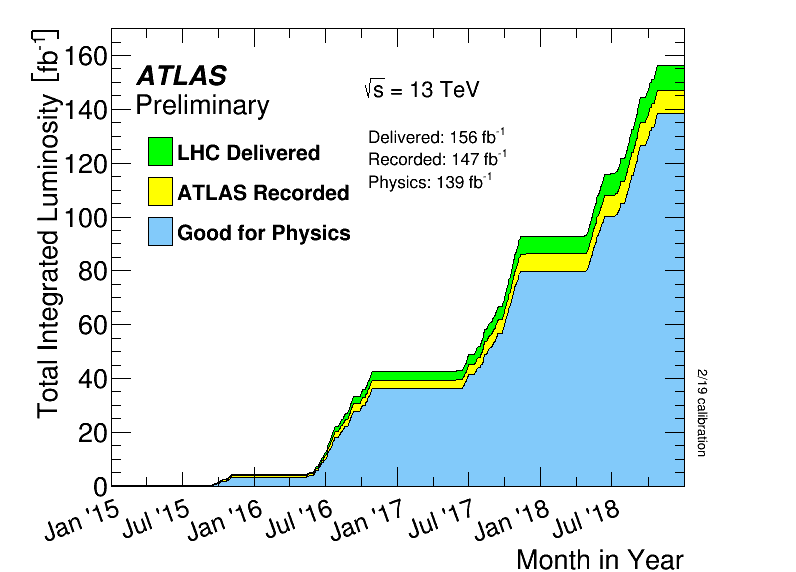
\includegraphics[width=0.6\textwidth]{Ch2/Img/Lumi.png}
    \caption{Luminosity delivered by the LHC during the Run 2 data taking. ATLAS recorded this data with an efficiency above 90\%.}
    \label{fig:chap2:LHC:Lumi}
\end{figure}
Knowing the cross section of the \HHyybb production, one can evaluate the number of events available for the analysis as $N_{HH\rightarrow\gamma\gamma\bar{b}b} = \mathcal{L}_{int}\cdot\sigma_{pp\rightarrow HH}\cdot Br(HH\rightarrow\gamma\gamma\bar{b}b)$ that leads to about 12 events.
\subsection{Pile-up}
\label{chap2:LHC:PU}
Because of the very high density of protons at the collision points, more than one proton interact when two LHC bunches cross each other at the center of the experiment. This is commonly referred to as pileup. On top of the usual $in-time$ pileup, defined as the collision events occurring during the same bunch-crossing as the event of interest, one also has to consider $out-of-time$ pileup, coming from remnants of information found in some of the detector subsystems that end-up being attributed to the wrong bunch-crossing, and therefore to the wrong event typically from previous collisions. Figure \ref{fig:chap2:LHC:PU} shows the average number of simultaneous interactions per bunch crossing for Run 2. \\
\begin{figure}[H]
    \centering
    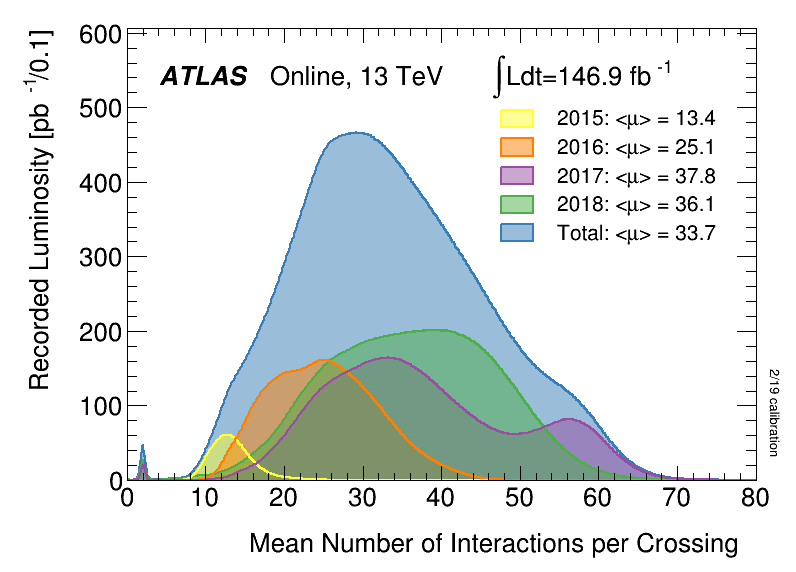
\includegraphics[width=0.6\textwidth]{Ch2/Img/PU.png}
    \caption{Mean number of interaction per bunch crossing in pp collisions recorded by the ATLAS detector during Run 2 at 13 TeV.}
    \label{fig:chap2:LHC:PU}
\end{figure}
The particles created in LHC collisions are distributed over the full solid angles around the Interaction Point (IP), in four IP point is installed four detectors to record those particles and identified them as ATLAS, CMS, ALICE and LHCb each is specific to study a category of physics. LHCb built to study flavour physics looking at the properties of b-hadrons, and the ALICE detector that is specialised for measurements on heavy-ion collisions. CMS and ATLAS are general-purpose detectors. They allow to make precision measurements of SM processes, including the properties of the Higgs boson, and to search for physics beyond the SM. Next section is dedicated to ATLAS detector as the thesis is done withing ATLAS collaboration.

\section{ATLAS A Toroidal LHC ApparatuS detector}
\label{chap2:ATLAS}
ATLAS detector is one of the four experiments placed on the four crossing points of the LHC beams. It is currently the largest experiment of particles 46 m long and 25 m of diameter and more than 7000 tons of weight. It is a superposition of four sub-detectors, each optimized for the identification and the measurement of a specific category of particles : Inner Tracker, Electromagnetic Calorimeter (ECAL), Hadronic Calorimeter  (HCAL) and Muons Spectrometer. It is composed of central called Barrel and two End-Cap to cover the $4\pi$ solid angle. The detector has been operating since 2008, taking alignment data with cosmic rays before the LHC launch, and its data is exploited by a collaboration of about 3000 scientific authors from 181 institutions in 38 countries. An overview sketch of the ATLAS detector is shown in Figure \ref{fig:chap2:ATLAS:Img}.
\begin{figure}[H]
    \centering
    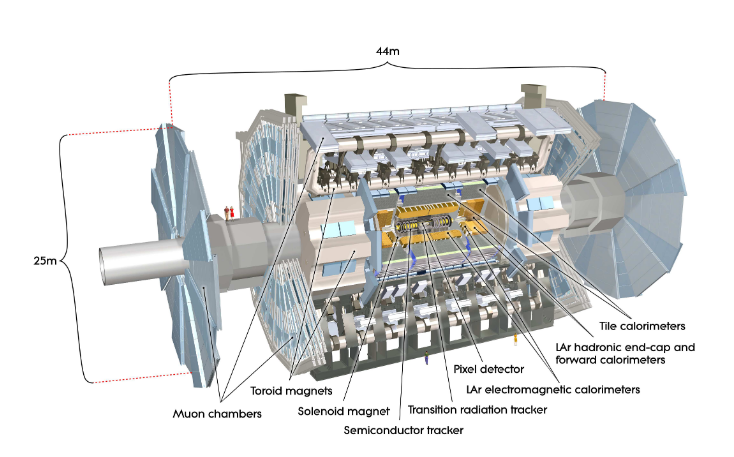
\includegraphics[width=0.8\textwidth]{Ch2/Img/ATLAS_sketch.png}
    \caption{Sketch of the ATLAS detector with its different sub-detectors.}
    \label{fig:chap2:ATLAS:Img}
\end{figure}

\subsection{Coordinated system}
\label{chap2:ATLAS:CS}
The coordinate system used in the ATLAS experiment is cylindrical coordinates with the z-axis is the LHC beam pipe, the x-axis pointing toward the center of the LHC ring and the y-axis pointing upward. A physic object (particle) is identified by its transverse competent of the three-momentum $p_T = \sqrt{p_X^2 + p_Y^2}$, its azimuthal angle $\phi \in [-\pi,\pi] $ formed by the three-momentum and the x-axis and its polar angle $\theta \in [0,\pi]$, i.e the angle between the three-momentum and the z-axis. \\
The polar angle is expressed in terms of the pseudo-rapidity $\eta$, defined as
\begin{equation}
\eta = -\log[\tan(\theta/2)].
\end{equation}
In protons collisions, the adoption of $\eta$ instead of $\theta$ ensure the detector balance over particles and particles distribution recorded is approximately flat with respect to $\eta$.
\begin{equation}
\frac{\partial\sigma_{QCD}}{\partial\eta} = cte.
\end{equation}
The pseudo-rapidity $\eta$ coincides for relativistic particles to the rapidity $y$, defined as 
\begin{equation}
y = \frac{1}{2}(\frac{E+p_Z}{E-p_Z}),
\end{equation}
where E is the particle energy.
Figure \ref{fig:chap2:ATLAS:SYS} shows the coordinate system common by ATLAS and CMS experiments.
\begin{figure}[H]
    \centering
    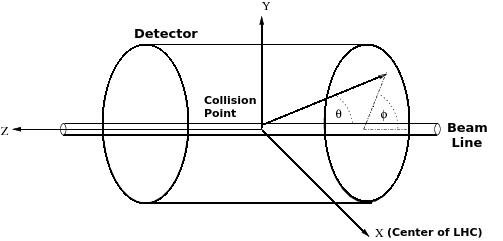
\includegraphics[width=0.6\textwidth]{Ch2/Img/ATLAS_Sys.jpeg}
    \caption{Coordinate system used by the ATLAS and CMS experiments at the LHC.}
    \label{fig:chap2:ATLAS:SYS}
\end{figure}

\subsection{The Inner Tracker}
\label{chap2:ATLAS:ITk}
The Inner Detector (ID) has been designed to detect and reconstruct the path of the electrically charged particle bent by a 2T solenoid magnetic field, and provides an excellent momentum  resolution by reconstructing curvature and direction, and both primary and secondary vertex measurements for tracks above approximately 0.5 GeV. In terms of acceptance, the ID cover region of $|\eta|\leqslant2.5$. To achieve the momentum and vertex resolution requirements imposed by the physics goals at the LHC and the very large track density environment, the ID high-precision measurements must be made with fine detector granularity. The ID is composed of four complementary sub-detectors: IBL, the Pixel Detector, the Semi Conductor Tracker (SCT) and the Transition Radiation (TRT). The magnetic field of 2 T is provided by a solenoid inserted between the ID and the EM calorimeter. The layout of the Inner Detector (ID) is illustrated in Figure \ref{fig:chap2:ATLAS:ITK:ID}.
\begin{figure}[H]
    \centering
    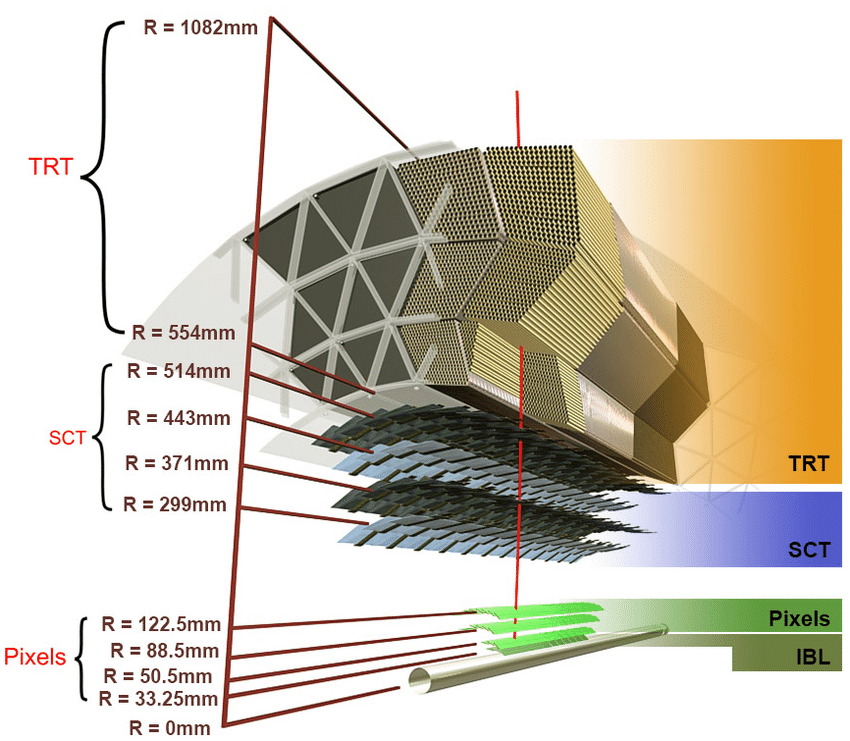
\includegraphics[width=0.5\textwidth]{Ch2/Img/ID_withIBL.png}
    \caption{Layout of the Inner Detector (ID), including the new Insertable B-Layer (IBL)}
    \label{fig:chap2:ATLAS:ITK:ID}
\end{figure}
\subsubsection{IBL}
\label{chap2:ATLAS:ITK:IBL}
In 2014, at the first LHC long shutdown, the ATLAS pixel detector was complete with a pixel layer installed close to the beam pipe called Insertable B-Layer (IBL). It means motivations are :
\begin{itemize}
	\item Insure the good identification of the primary vertex which play an important role in $b$-jet identification ($b$-tagging), which in turn significantly improves the sensitivity of many analyses. Inefficiencies in the other layers can be partially compensated during reconstruction at the cost of an increased fake rate, the IBL restore the full $b$-tagging efficiency even in case of a complete B-layer failure.
	\item Luminosity effects, The current pixel detector was designed for a peak luminosity of $10^{34} cm^{-2}s^{-1}$. With high luminosity the event pileup is increased, leading to high occupancy that can induce readout inefficiencies, would thereby limit the $b$-tagging efficiency. The addition of the IBL layer helps to preserve tracking performance in face of luminosity effects.
\end{itemize}
Strong constraints and project specifications have a substantial impact on the technologies required for the IBL. IBL covers the region of $|\eta|< 2.58$ in pseudo-rapidity and located at a mean radius of 33.2 mm around the beam pipe. The pixels uses 12 million pixels with a typical size of 50x250 $\mu$m. The IBL consists of 14 staves with each 20 modules made using either planar or 3D sensors. The temperature of the IBL is controlled using a bi-phase CO2 cooling system. Figure \ref{fig:chap2:ATLAS:ITK:IBL} shows the IBL within the Pixel Detector volume and around the beam pipe.
\begin{figure}[H]
    \centering
    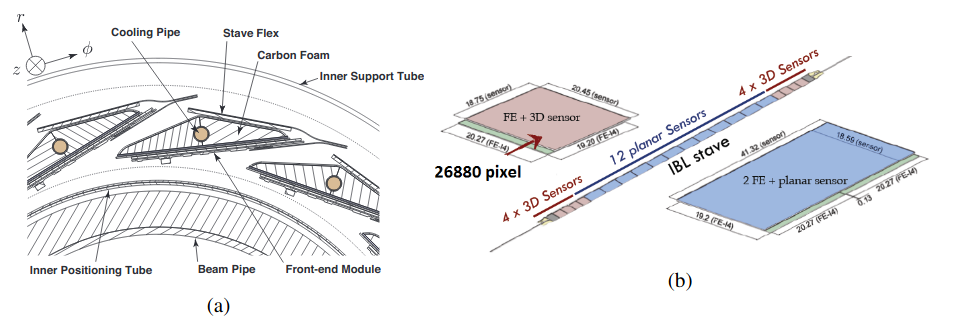
\includegraphics[width=0.8\textwidth]{Ch2/Img/IBL.png}
    \caption{(a) Transverse view of 3 of the Insertable-B-Layer (IBL) staves, located directly on the beam pipe. (b) The layout of one of the 14 IBL staves.}
    \label{fig:chap2:ATLAS:ITK:IBL}
\end{figure}

Additional measurement point provided by IBL improves significantly the tracking. Figure \ref{fig:chap2:ATLAS:ITK:IBL:Imp} shows the improvement in impact parameter resolution due to the IBL as measured from early Run 2 data with respect to Run 1. 
\begin{figure}[H]
    \centering
    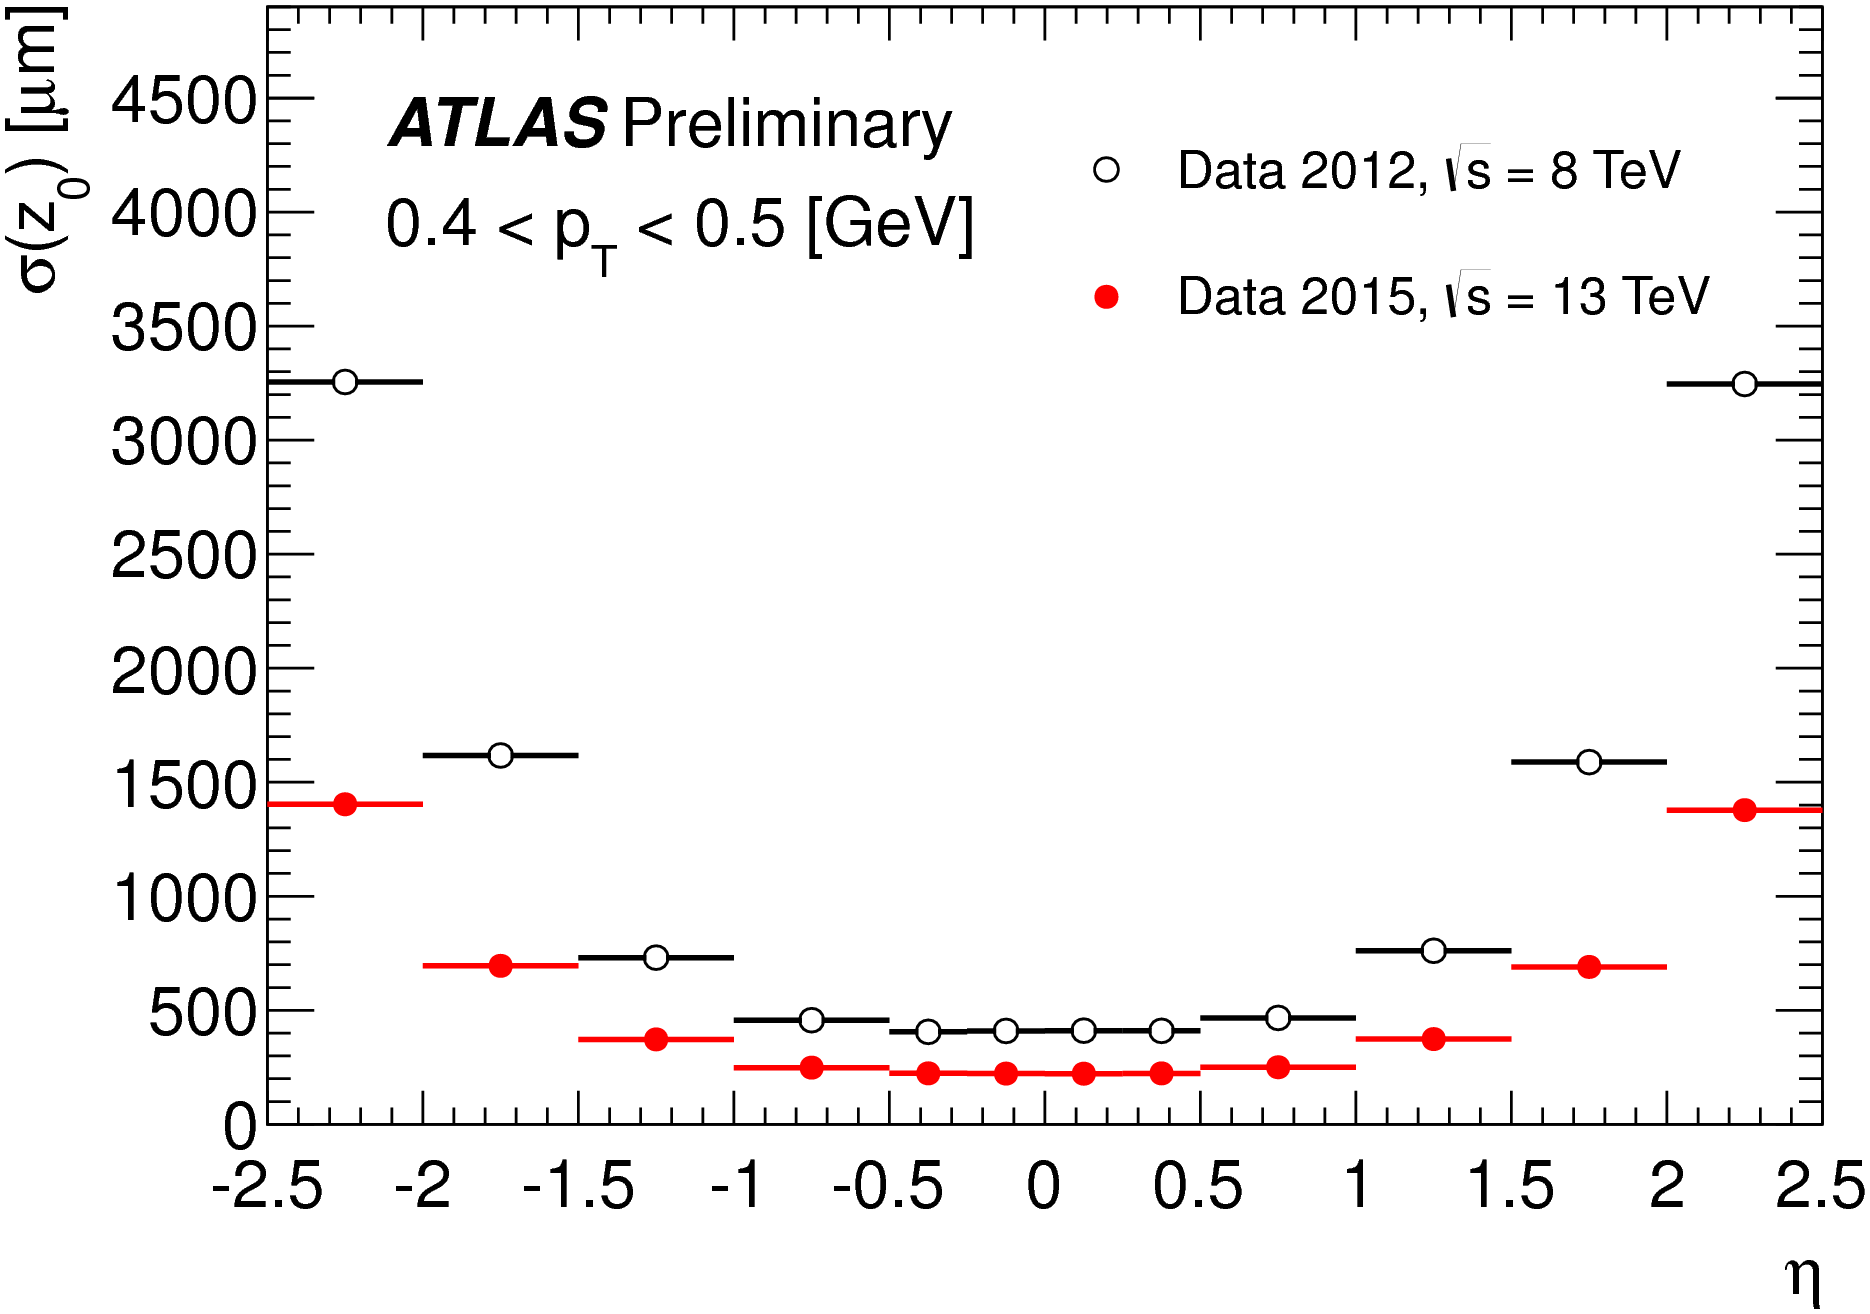
\includegraphics[width=0.6\textwidth]{Ch2/Img/IBL_impact.png}
    \caption{Unfolded longitudinal impact parameter resolution measured from data in 2015, $\sqrt{s}= 13$ TeV, with the Inner Detector including the IBL, as a function of $\eta$  for values of 0.4 < \pT < 0.5 GeV compared to that measured from data in 2012, $\sqrt{s} = 8$ TeV.}
    \label{fig:chap2:ATLAS:ITK:IBL:Imp}
\end{figure}
In addition, Figure \ref{fig:chap2:ATLAS:ITK:IBL:Trk} shows the improvement achieved with IBL for the performance of tracking in dense environments (TIDE). Improvements in tracking  have a direct impact on vertex identification and $b$-tagging. 
\begin{figure}[H]
    \centering
    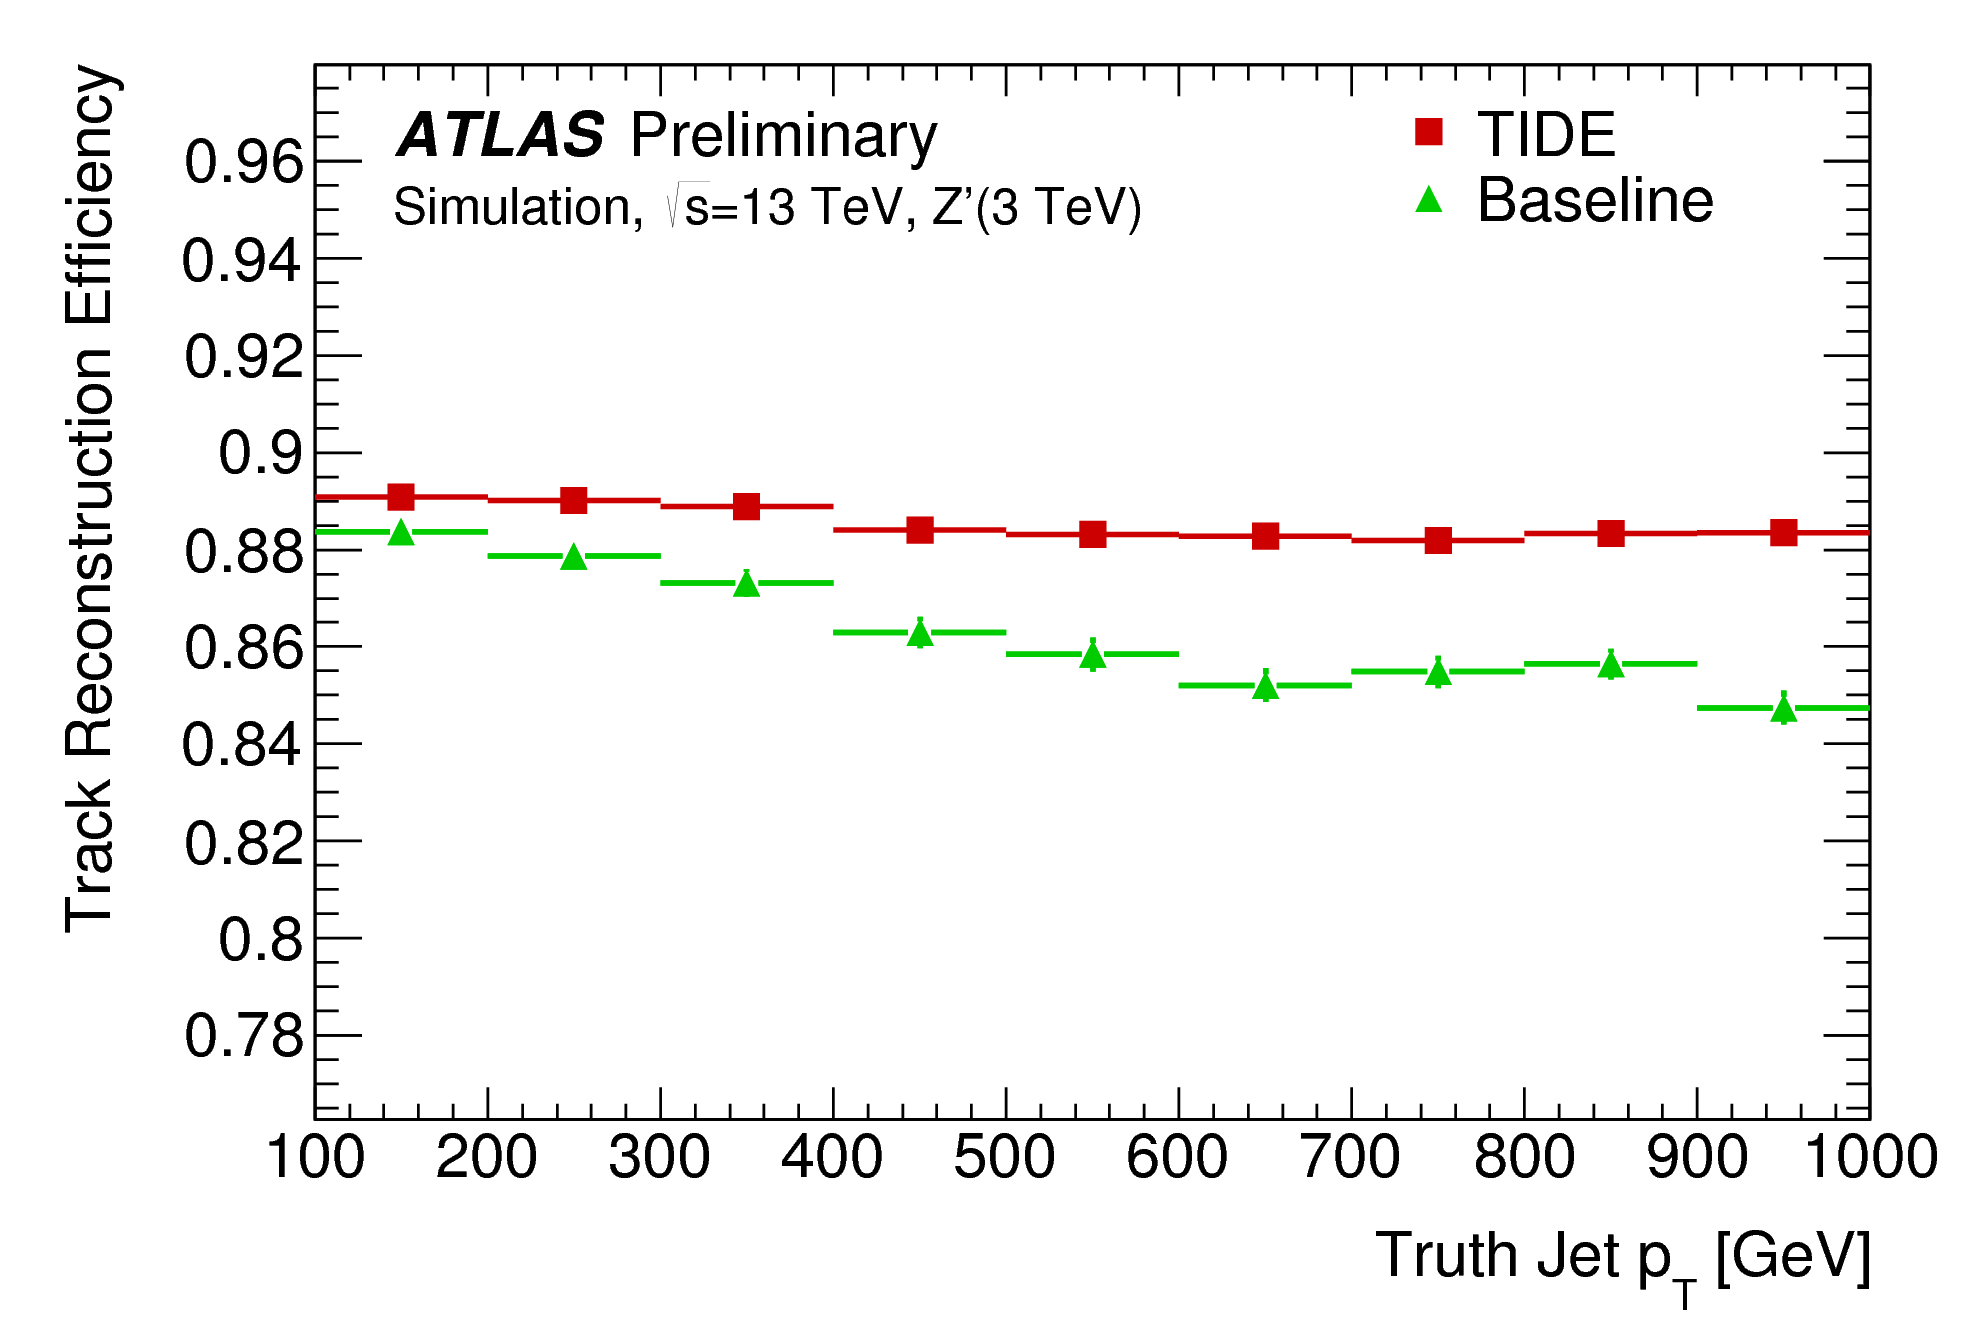
\includegraphics[width=0.6\textwidth]{Ch2/Img/IBL_track.png}
    \caption{The average efficiency to reconstruct primary tracks with a production vertex before the first layer in jets as a function of jet \pT. The same sample generation, with limited statistics, is used for both reconstruction algorithms resulting in correlated features.}
    \label{fig:chap2:ATLAS:ITK:IBL:Trk}
\end{figure}
Figure \ref{fig:chap2:ATLAS:ITK:IBL:Btag} shows the improvement in the $b$-tagging efficiency with IP3D+SV1 $b$-tagging algorithms respect to Run 1 algorithm due to the IBL. The IP3D and SV1 algorithms will be explained later in the thesis.
\begin{figure}[H]
    \centering
    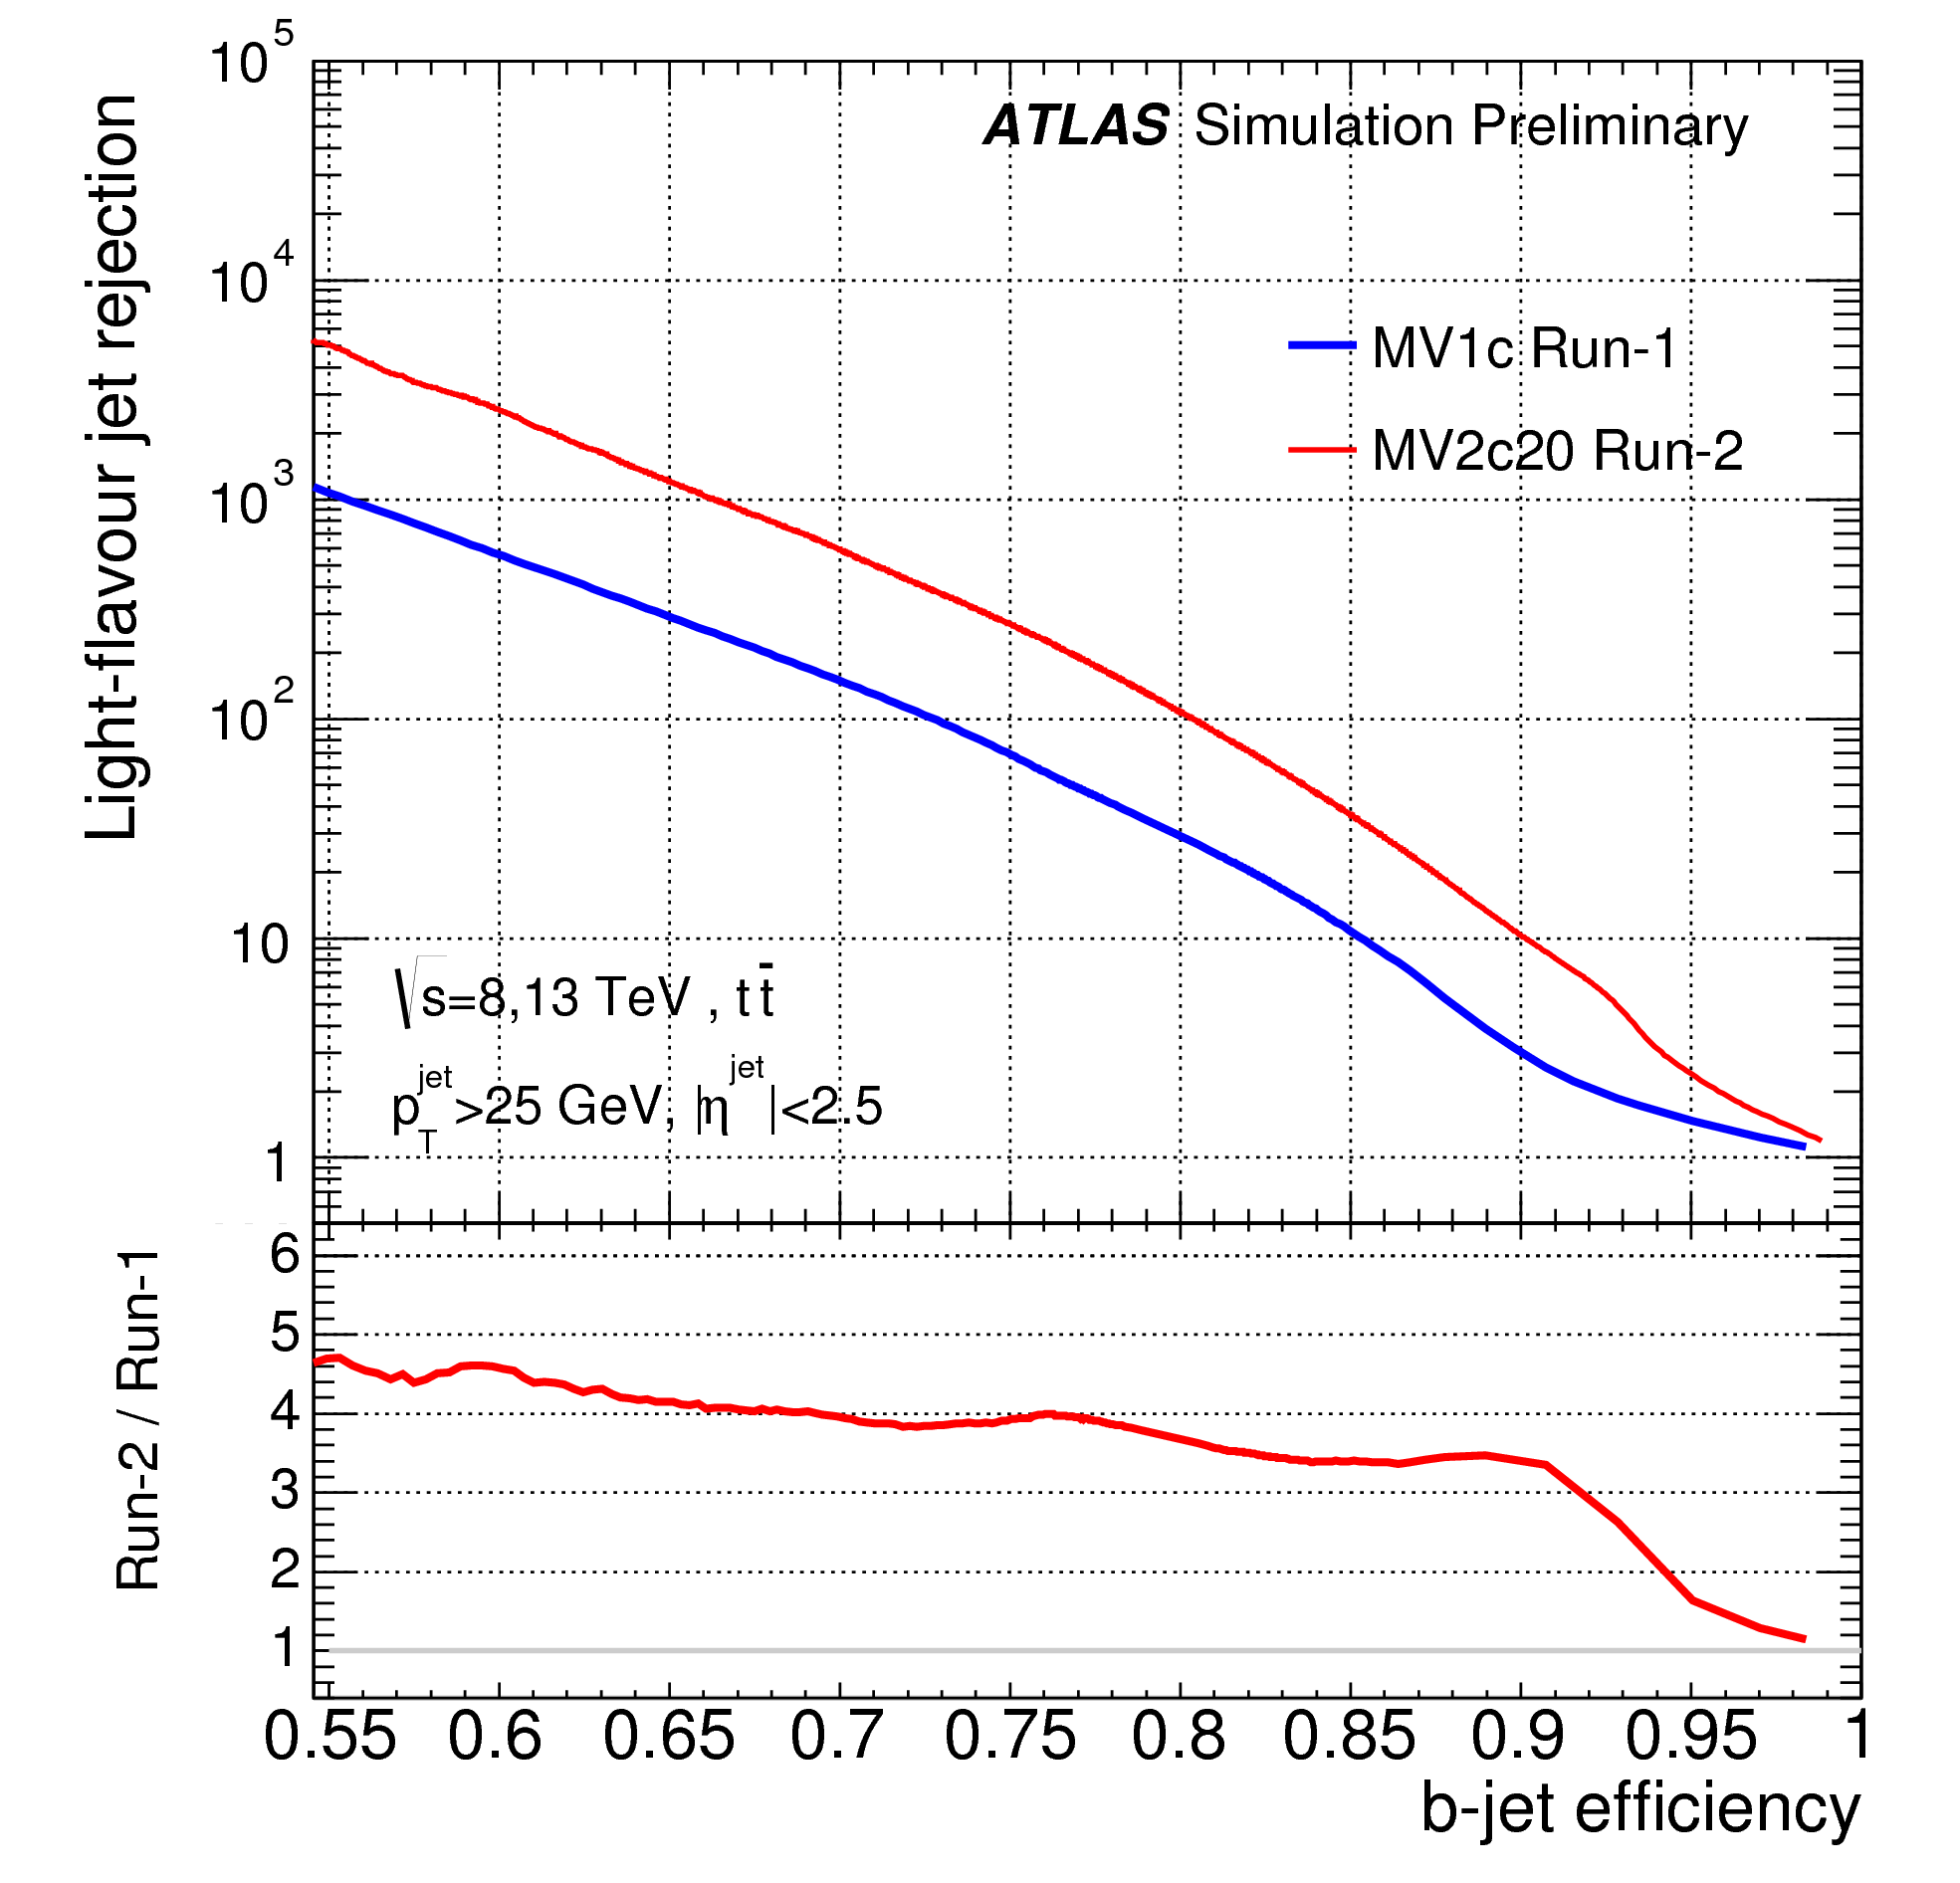
\includegraphics[width=0.6\textwidth]{Ch2/Img/IBL_btag2.png}
    \caption{Rejection factor against light jets as a function of $b$-jet efficiency for t the combined IP3D+SV1 tagger. Compared are the results with and without IBL.}
    \label{fig:chap2:ATLAS:ITK:IBL:Btag}
\end{figure}
\subsubsection{Pixel Detector}
\label{chap2:ATLAS:ITK:PD}
The Pixel Detector (PD) is designed to provide high-granularity, high-precision measurements as close as possible to the interaction point (IP). It consists of three barrel layers placed at the radius of 50.5 mm , 88.5 mm and 122.5 mm centered around the beam axis and two end-cap with three disc layers each positioned at $|z|= 495.580$ and $650 \ mm$. It provides three measurement points per track. The system is designed to be highly modular, containing approximately 1500 identical barrel modules and 1000 identical disk modules, each module is composed of 61440 pixel elements of silicon semi-conductor. In total there are about 80 million readout channels in the whole PD. The spatial resolution for the barrel modules is 10 $\mu$m in r-$\phi$ and 66 $\mu$m in z, for the end-caps the spatial resolution in r-$\phi$ is same as the barrel and 115$\mu$m in r. The main limitation of the pixel detector is the radiation hardness as the expected flounce is at the tolerable limit. 
\subsubsection{Semi Conductor Tracker}
\label{chap2:ATLAS:ITK:SCT}
The SCT system is designed to provide four precision points per track in the intermediate radial range, contributing to the measurement of momentum, impact parameter and vertex position. The barrel and end-caps SCT are four layers of silicon microstrip for barrel and nine disks for end-caps. The spatial resolution is 16 $\mu$m in r-$\phi$ for both the barrel and the end-caps. The four complete barrels are positioned in radius of 300, 373, 447 and 520 mm. Tracks can be distinguished if separated by more than $\sim$200 $\mu$m. There are 6.3 millions readout channels for the SCT.
\subsubsection{Transition Radiation Tracker}
The TRT occupies the other part of the ID. It consist of 370000 drift tubes called straws, each straw has a diameter of 4 mm and 1.44 m in long. The straws are filled with gas mixture of 70\% $Xe$, 27\% $CO_2$ and 3\% $O_2$ its wall acts as a cathode and kept at high voltage. The anode is a 30 $\mu$m diameter plated tungsten wire placed in the center of the straw. When a charged particle traverses a straw, it ionizes the gas and the produced electrons travel through the anode generating an electric signal. To keep the TRT performance to be constant, the close-loop gas system is used maintaining the correct gas fractions. The straws are arranged to be parallel to the beam-pipe in the barrel and perpendicular in the end-cap region. There are about 50k straws in the barrel and 320k straws in the end-cap providing high precision measurement for each track. The radial resolution is about 130 $\mu m$. \\
In the Perigee representation, tracks are described using the parameters of a helical trajectory at the point of closest approach to the z-axis: the transverse impact parameter $d_0$, the z coordinate $z_0$, the angles $\theta$ and $\phi$ and the inverse of the particle momentum multiplied by the charge q/p, as illustrated in Figure \ref{fig:chap2:ATLAS:ITK:Trk}
\begin{figure}[ht]
    \centering
    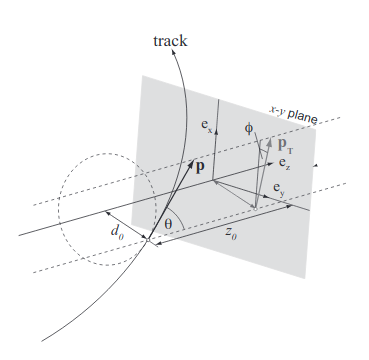
\includegraphics[width=0.5\textwidth]{Ch2/Img/Track.png}
    \caption{The Perigee representation of the track.}
    \label{fig:chap2:ATLAS:ITK:Trk}
\end{figure}
The expected momentum resolution of the inner detector, without the IBL, is given by:
\begin{equation}
    \sigma(1/p_T)\cdot p_T = 0.036\%\cdot p_T [GeV] \oplus 1.3\%,
\end{equation}
$\oplus$ denote the quadrature addition.
\subsection{Calorimeter system}
\label{chap2:ATLAS:Calo}

Based on the calorimetry, the ATLAS calorimeter system is designed to provide a precise energy and position reconstruction for electromagnetic particles (electrons, photons) and jets (hadrons). The calorimeter also allows to measure the missing transverse energy and provides the separation of electrons and photons from hadrons and jets. The calorimeter system is composed of two calorimeters: the electromagnetic calorimeter (ECal) and the hadronic calorimeter (HCal). Both of them are sampling calorimeters, with alternating layers of a heavy absorber material and an active material in which an ionisation signal is produced. Figure \ref{fig:chap2:ATLAS:Calo} shows a three dimensional view of the ATLAS calorimeter system.
\begin{figure}[H]
    \centering
    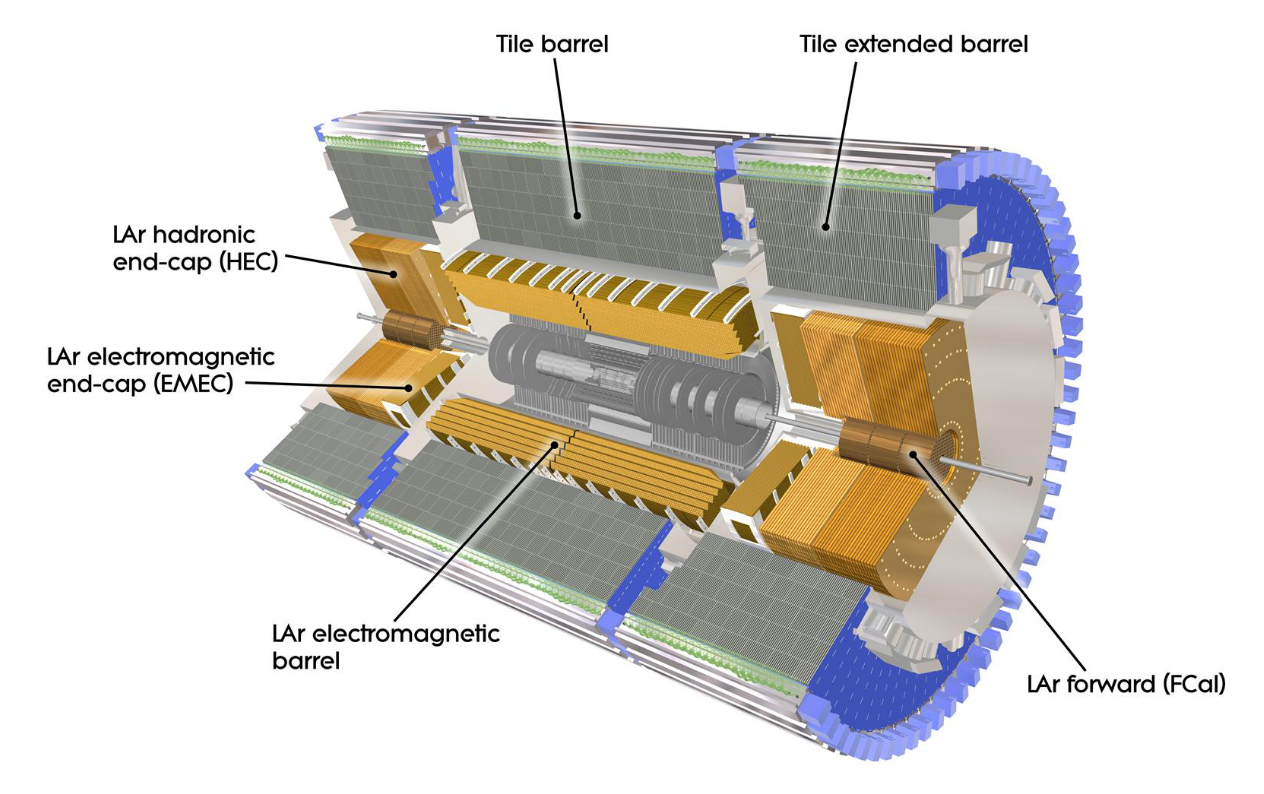
\includegraphics[width=0.6\textwidth]{Ch2/Img/Calo.png}
    \caption{ATLAS Calorimeter system.}
    \label{fig:chap2:ATLAS:Calo}
\end{figure}

\subsubsection{Electromagnetic calorimeter}
\label{chap2:ATLAS:Calo:ECAL}
The ECal is the first sub-detector after the ID. Is dedicated to reconstructing the energy of electrons and photons exploiting their showers. It covers the region of $|\eta|<$3.2 excluding the region 1.375 $<|\eta|<$ 1.52 which correspond to the transition region between the barrel and end-caps. The barrel part covers $|\eta|<$1.475, while the two end-caps cover 1.375$<|\eta|<$3.2. The barrel and end-caps are composed of alternated layers of absorbing material Lead (Z=82), separated by active medium Liquid Argon (LAr). The advantages of LAr, such as radiation hardness, intrinsic linear behaviour, cheapness compared to other noble gases, have been considered to outweigh the difficulties associated with the need of cryostats and signal feed-throughs. The total thickness of the calorimeter is 22 radiation lengths in the barrel, and more than 24 radiation lengths in the end-caps. The radiation lengths $X_0$ is defined as the scale after which high-energy electrons loose all but 1/e of their initial energy. $X_0$ of lead is 5.6mm. \\
Electrons and photons traversing the calorimeters initiate electromagnetic cascades, in which $e^+e^-$ pair production and bremsstrahlung processes occur. High-energy electrons predominantly loose energy in matter through bremsstrahlung, while high-energy photons create $e^+e^-$. EM particle produce shower when passed through ECal until its energy falls below the critical energy $E_c$. $E_c$, can be defined as the energy for which the energy loss per $X_0$ due to ionisation of the material is equal to the particle energy. In lead, $E_c$=7.4 MeV for electrons. The EM shower ionizes the atom of the liquid Argon generating an electric signal proportional to the energy deposit by the particle. The ionization is drifted to the electrode under electric field generated by the high voltage of 2000 V. To provide a huge signal response and hermiticity, ATLAS Collaboration adopted a particular geometry for the ECal: $accordion$ geometry. In the barrel, the accordion waves are axial and run in $\phi$; the folding angles of the waves vary with radius to keep the liquid-argon gap constant and reduce the died zone. In the end-caps, the waves are parallel to the radial direction and run axially. The size of the drift gap on each side of the electrode is 2.1 mm. Figure \ref{fig:chap2:ATLAS:Calo:ECal:Acc} shows the accordion shape of the EM calorimeter.
\begin{figure}[H]
    \centering
    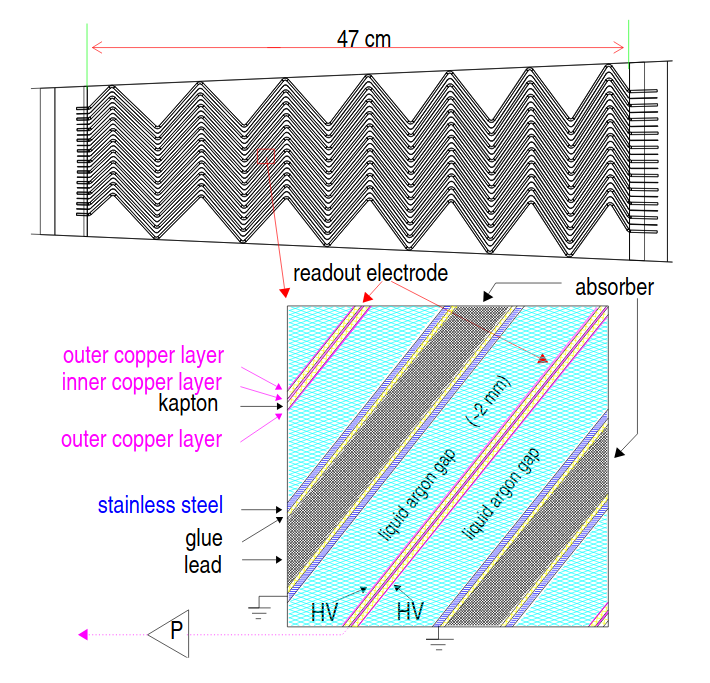
\includegraphics[width=0.6\textwidth]{Ch2/Img/ECal_accord.png}
    \caption{Accordion shape of the EM calorimeter.}
    \label{fig:chap2:ATLAS:Calo:ECal:Acc}
\end{figure}
The ECal is further segmented in three longitudinal layers, to allow to measure the longitudinal shower development called respectively strip, middle and back. It has different EM cells granularity $\Delta\eta\times\Delta\phi$ per layer. Cells of the middle layer (Lr2) in the barrel region are $0.025\times0.025$, while for the strip (Lr1) cells are 8 times finer in the $|\eta|$ direction providing a precise $\eta$ measurement of incident particles. The back layer (Lr3) cells has a twice coarser granularity in $\eta$ and the same $\phi$ segmentation as in Lr2. Before the EM barrel calorimeter there is a Presampler (PS) LAr detector (Lr0) ,covering range $|\eta|<$1.8 and placed placed to start the shower before the calorimeter. PS has the finest granularity with a cell size of $\Delta\eta\times\Delta\phi = 0.003\times0.1$ used for $\pi\rightarrow\gamma\gamma$ background separation. The number of samplings  and the granularity in each of the samplings are summarized in Table \ref{tab:chap2:ATLAS:Calo:ECal:Gr}.
\begin{table}[ht]
    \centering
    \begin{tabular}{cccccc}
    \hline
    Sampling & $|\eta|<$1.5 & 1.5$<|\eta|<$1.8 & 1.8$<|\eta|<$2.0 & 2.0$<|\eta|<$2.5 & 2.5$<|\eta|<$3.2 \\
    \hline
    \hline
        Presampling & 0.025$\times$0.1 & 0.025$\times$0.1  \\
        Strip & 0.025/8$\times$0.1 & 0.025/8$\times$0.1 & 0.025/6$\times$0.1 & 0.025/4$\times$0.1 & 0.1$\times$0.1 \\
        Middle & 0.025$\times$0.025 & 0.025$\times$0.025 & 0.025$\times$0.025 & 0.025$\times$0.025 & 0.1$\times$0.1 \\
        Back & 0.050$\times$0.025 & 0.05$\times$0.025 & 0.05$\times$0.025 & 0.05$\times$0.025 \\
        \hline
    \end{tabular}
    \caption{Granularity of the EM calorimeter ($\Delta\eta\times\Delta\phi$)}
    \label{tab:chap2:ATLAS:Calo:ECal:Gr}
\end{table}
Physics studies showed that precision physics can hardly be extended beyond a pseudorapidity of 2.5. For this reason, the small wheel has a coarser granularity and only two samplings in depth. EM calorimeter resolution is given by:
\begin{equation}
    \sigma_E/E = \frac{10\%}{E} \oplus 0.17\%.
\end{equation}
\subsubsection{Hadronic calorimeter}
\label{chap2:ATLAS:Calo:HCAL}


